\documentclass{article}
\usepackage{microtype}
\usepackage{graphicx}
\usepackage{subcaption}
\usepackage{booktabs}
\usepackage{hyperref}
\newcommand{\theHalgorithm}{\arabic{algorithm}}
\usepackage{icml2026}
\usepackage{amsmath}
\usepackage{amssymb}
\usepackage{mathtools}
\usepackage{amsthm}
\usepackage[capitalize,noabbrev]{cleveref}
\graphicspath{{../results/figs/}}
\newcommand{\phihat}{\hat{\boldsymbol\phi}}
\newcommand{\phivec}{\boldsymbol\phi}
\icmltitlerunning{How reliable is a single run of SHAP?}

\begin{document}

\twocolumn[
  \icmltitle{When Is One Run Enough? Repeat-Run Reliability of\\Sampling-Based SHAP Attributions on Tabular Models}
  \begin{icmlauthorlist}
    \icmlauthor{Anonymous Authors}{anon}
  \end{icmlauthorlist}
  \icmlaffiliation{anon}{Anonymous Institution}
  \icmlcorrespondingauthor{Anonymous Authors}{anonymous@example.org}
  \icmlkeywords{SHAP, Shapley values, explanation stability, tabular data, KernelSHAP, reproducibility}
  \vskip 0.3in
]
\printAffiliationsAndNotice{}

\begin{abstract}
SHAP attributions are routinely computed once per instance with a randomised estimator under a fixed compute budget and then used as the stated reason for a prediction. We ask when such a single run is a reliable basis.
We re-run Kernel- and permutation-sampling Shapley estimators many times for the same model, instance and background on four public tabular datasets ($d=8$--$20$) and four model classes, at budgets from $2d$ to $64d$ coalition evaluations, and compare run-to-run disagreement with exact attributions and with three other sources of variation (model retraining, background resampling, value-function choice).
The answer is conditional.
With a \emph{fixed background}, a single run recovers the top-1 feature (two-run agreement $\ge0.9$) for 81--92\% of instances at $8d$--$16d$ evaluations (pooled over cells), but identifies the top-3 \emph{set} reliably for only 57--71\%; errors concentrate in instances whose attribution margins are small relative to noise, not in particular datasets or budgets.
With shap's default settings and a \emph{resampled background}, which is common practice, single-run top-3 sets are reproducible for only 29--42\% of instances, and background resampling dominates coalition-sampling noise.
A permutation run's own pair-level statistics give a calibrated single-run certificate (top-1 accuracy $0.93\!\to\!0.98$ at 78\% coverage for $m=4d$), and splitting a permutation budget into repeat runs costs nothing in accuracy whereas splitting a Kernel budget does.
\end{abstract}

\section{Introduction}
Shapley-value attributions \citep{shapley1953,lundberg2017} are used to justify individual decisions in credit, health and similar settings.
For models that are not trees or linear, they are \emph{estimated}: Kernel SHAP and permutation sampling draw random coalitions or permutations and evaluate the model on a limited number of them \citep{lundberg2017,mitchell2022,covert2021}.
Two runs on the same trained model, instance and background therefore return different attribution vectors, yet the common practice is one run per instance, with the resulting ranking or top features reported as the rationale for the prediction.
Prior work establishes that estimators converge, with variance and, recently, non-asymptotic guarantees on $\ell_2$ error \citep{covert2021,musco2024}, and that explanations can disagree across methods \citep{krishna2022}, backgrounds \citep{yuan2022} or perturbations \citep{alvarezmelis2018,ghorbani2019}.
What is missing for a practitioner is a direct answer to a decision-level question: \emph{at the budget I can afford, is the explanation I just computed what I would get if I ran it again, and compared with what other uncertainty sources, does it matter?}

We study this question empirically with a design chosen to make the answer falsifiable.
Reliability is operationalised at the level at which explanations are used (top-1 feature, top-$k$ set, ranking, sign), not only $\ell_2$ error (\cref{sec:method}); every number is compared with exact Shapley values where they can be computed and with ``yardsticks'' from other sources of explanation variability.
Our contributions are:
\begin{enumerate}
\item \textbf{A protocol} (budget in units of $d$ coalition evaluations; repeated-run agreement metrics; yardsticks; instance-clustered uncertainty) and a re-implementation of shap's Kernel and permutation estimators, validated against the package (\cref{sec:validation}), with exact $2^d$ coalition tables that make $\sim\!10^6$ estimator runs cheap.
\item \textbf{Evidence on conditions.} Across 4 datasets, 4 model classes, 2 estimators and 6 budgets we report when a single run is enough for which downstream use, and show that reliability is governed by the instance's \emph{margin-to-noise ratio} rather than by dataset or budget alone.
\item \textbf{Practice-relevant findings:} shap's default KernelExplainer is exactly reproducible for $d\le10$ on a fixed background, so most observed run-to-run variation in default pipelines comes from background resampling and from the default permutation budget; and a permutation run can certify its own top-$k$ ranking.
\end{enumerate}
We state the claims in \cref{sec:claims} and report negative and inconclusive results in \cref{sec:results,sec:limits}.

\section{Related Work}
\textbf{Estimating Shapley values.} Kernel SHAP casts Shapley values as a weighted regression over sampled coalitions \citep{lundberg2017}; \citet{covert2021} analyse its variance, give convergence detection and uncertainty estimates and a paired-sampling variance reduction; permutation sampling with antithetic or quasi-Monte-Carlo schemes is studied by \citet{mitchell2022}; Leverage SHAP gives non-asymptotic guarantees for a Kernel-SHAP variant \citep{musco2024}; TreeSHAP is exact for trees \citep{lundberg2020trees}. These works optimise or bound \emph{estimation error}; we measure \emph{decision-level reproducibility} of the deployed estimators at small budgets and relate it to other explanation uncertainties. Our single-run certificate (\cref{sec:cert}) is a rank-level use of the variance information that \citet{covert2021} propose for feature-wise uncertainty; we do not claim the idea of in-run uncertainty as new, only its empirical calibration for top-$k$ claims.

\textbf{Explanation stability and disagreement.} Explanations differ across methods \citep{krishna2022}, are sensitive to input perturbation \citep{alvarezmelis2018,ghorbani2019}, can be manipulated \citep{slack2020}, and depend on the value function, i.e.\ whether expectations are taken ``true to the model or true to the data'' \citep{chen2020,janzing2020,kumar2020}. \citet{yuan2022} show for deep models on one clinical dataset that SHAP values and rankings change with the random background sample. We take background resampling as one of several yardsticks across four datasets and four model classes, alongside estimator randomness. \textbf{Model multiplicity.} Equally accurate models can give different predictions or variable importances \citep{marx2020,fisher2019}; we use retraining variability as a yardstick for how much explanation instability is already unavoidable. \textbf{Stability measures.} We use Jaccard and the Nogueira et al.\ stability of selections \citep{nogueira2018} and rank-biased overlap \citep{webber2010}.

\section{Method}\label{sec:method}
\textbf{Setting.} A trained model $f:\mathbb{R}^d\to[0,1]$ gives $P(y{=}1\mid x)$, with $d$ attributes (one-hot columns of a categorical attribute form one player). For instance $x$ and background set $\mathcal{B}$ of $B{=}100$ training rows, the interventional value function is $v(S)=\frac1B\sum_{b\in\mathcal B}f(x_S,b_{\bar S})$ and $\phivec$ is its Shapley value. This is the value function behind shap's Kernel/Permutation explainers and interventional TreeSHAP \citep{chen2020,lundberg2020trees}. Attributions are ranked by $|\phi_j|$.

\textbf{Estimators and budget.} \emph{Kernel}: shap's allocation of $m$ distinct coalitions (full enumeration of the cheapest paired size strata, then random paired sampling; weighted least squares with the efficiency constraint). \emph{Permutation}: antithetic (forward+reverse) permutation sampling; one pair costs $2(d{-}1)$ coalition evaluations, so $\lfloor m/(2(d{-}1))\rfloor$ pairs are used. Budget $m$ is the number of coalition evaluations (each is $B$ model calls) and is reported as $m/d\in\{2,4,8,16,32,64\}$ ($\le32$ for $d{=}20$); $m\ge2^d-2$ makes Kernel exact. A ``run'' differs from another only in the estimator's random seed (model, instance, background fixed). Because $v$ for $d\le12$ is tabulated once ($2^d\!\cdot\!B$ model calls per instance), exact Shapley values and thousands of runs per instance are available; for $d{=}20$ the model is called live and the reference is the mean of 20 permutation runs of $64d$ evaluations each (an approximation, whose limits are noted in \cref{sec:limits}).

\textbf{Reliability metrics.} For two independent runs $\phihat,\phihat'$: top-1 agreement; top-3 set identity and Jaccard (also $k{=}5$); RBO ($p{=}0.9$, extrapolated) and Kendall $\tau$ of the $|\phi|$ rankings; relative $\ell_2$ difference; sign agreement among the shared top-3. The estimate for an instance averages 300 random pairs among $R$ runs ($R{=}50$; $30$ for $d{=}20$). Against the exact reference we also report top-1/top-3 accuracy and relative error.
\emph{Pre-specified primary outcome (before the full run):} an instance \emph{passes} for a use if the probability that two independent runs agree on it is $\ge0.9$ (top-1 feature, or identical top-3 set); the \emph{pass rate} is the fraction of instances that pass. The threshold is a convention; \cref{app:thr} shows the ordering of conclusions is unchanged at $0.8$--$0.99$.

\textbf{Yardsticks.} To judge whether a given disagreement matters we compute, on the same instances: (i) \emph{model retraining}: $K{=}5$ models retrained on bootstrap resamples, with exact attributions; (ii) \emph{background resampling}: 10 random backgrounds of size $B\in\{10,50,100,200\}$, exact attributions; (iii) \emph{value function}: path-dependent TreeSHAP vs.\ interventional (trees); (iv) \emph{between-instance} attribution distance (the spread any explanation must resolve); and (v) Kernel vs.\ permutation.

\textbf{Single-run diagnostics.} For $n\ge2$ antithetic pairs let $c_p\in\mathbb{R}^d$ be the pair-level contribution vectors, $\hat\phi=\bar c$. For the features $a,b$ ranked $r$ and $r{+}1$ by $|\hat\phi|$ with signs $s_a,s_b$, $z_r=\overline{D}/(s_D/\sqrt n)$ where $D_p=s_ac_{p,a}-s_bc_{p,b}$. A top-1 (top-3) claim is \emph{certified} if $z_1\ge1.96$ ($z_3\ge1.96$, separating ranks 3 and 4). We evaluate coverage and accuracy against the exact reference; thresholds are fixed a priori and never tuned. Alternatively, two half-budget runs \emph{agree}; and averaging $k$ runs of budget $m/k$ is compared with one run of budget $m$.

\textbf{Design.} Datasets: Pima ($d{=}8$), Give Me Some Credit (GMSC, $d{=}10$), ACSIncome (Colorado 2018, folktables \citep{ding2021}, $d{=}10$) and German Credit ($d{=}20$) \citep{german}. Models: logistic regression (LR), XGBoost \citep{chen2016xgboost}, random forest (RF) and a $2\times64$ MLP (sklearn \citep{pedregosa2011}); test AUC in \cref{app:models} (0.73--0.87). 100 random test instances per cell (50 for German), one trained model per cell for the main experiment. \emph{Statistics:} instance-level metrics are aggregated with percentile bootstrap CIs resampling instances (cells: resampling cells for pooled numbers); paired comparisons use Wilcoxon signed-rank tests with Holm correction \citep{wilcoxon1945,holm1979}. The pass criterion, $k{=}3$, the grid, the certificate thresholds and the claims below were fixed in the analysis design before the full runs (wording refined after a pilot with 6 instances and 10 runs per cell); all other analyses, including those of mechanism (\cref{sec:mech}), are exploratory and unadjusted unless a Holm correction is stated. We used ${\sim}$5 CPU-hours in total (\cref{app:repro}).

\section{Claims Under Test}\label{sec:claims}
\textbf{C1 (defaults).} With a fixed background and shap defaults, KernelExplainer is exactly reproducible for $d\le10$; most default-pipeline variability then comes from background resampling.
\textbf{C2 (budget/use).} For a fixed background and model, single-run reliability depends on the use: top-1 is reproducible for most instances at moderate budgets ($\gtrsim8$--$16d$), top-3 sets and rankings are not even at $64d$.
\textbf{C3 (conditions).} Instance-level unreliability is explained by small margin relative to noise (near-ties), is stronger for non-additive models and not specific to a dataset.
\textbf{C4 (yardsticks).} Sampling noise at $\ge16d$ is smaller than model-retraining variability; but not necessarily smaller than background-resampling variability.
\textbf{C5 (practice).} A single permutation run can certify its own top-$k$; splitting budgets is free for permutation, costly for Kernel.
Each is stated so that the tables below can refute it.

\section{Results}\label{sec:results}
\subsection{Validation of the re-implementation}\label{sec:validation}
On Pima (3 models, 10 instances each, 100 runs per setting, exact reference from the coalition table) the RMSE of our Kernel and permutation estimators matches \texttt{shap.KernelExplainer} (\texttt{l1\_reg=0}) and \texttt{PermutationExplainer} at equal evaluation budget (median ratios 1.00 and 0.97 for $m\ge4d$; \cref{app:valid}). At $m=2d$ both implementations produce unstable Kernel estimates: 14--23\% of random designs have an ill-conditioned normal-equation matrix (cond.\ $>10^8$; \cref{app:valid}), so $m=2d$ is below a usable budget for Kernel SHAP and is reported but not interpreted.

\begin{figure*}[t]
\centering
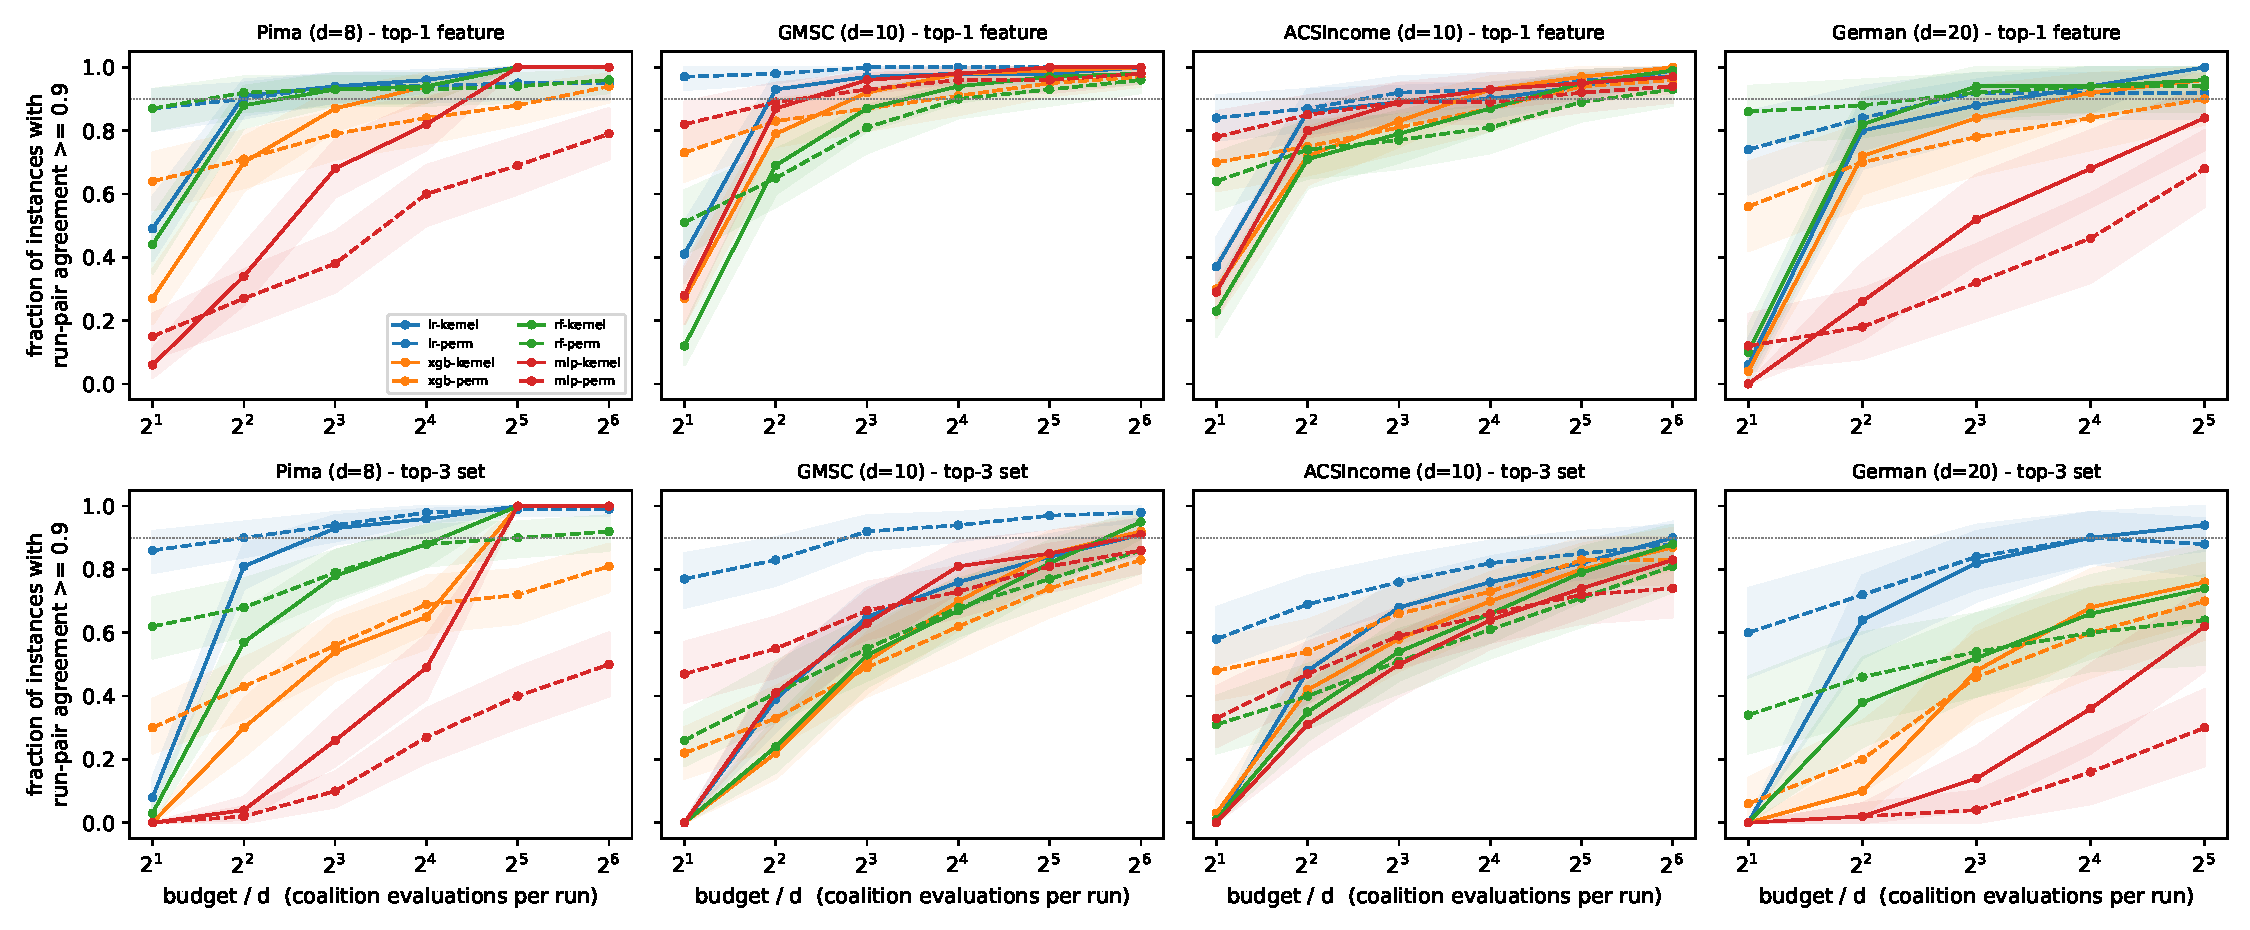
\includegraphics[width=\textwidth]{fig_passrate.pdf}
\caption{Fraction of instances whose two-run agreement is $\ge0.9$ (top: same top-1 feature; bottom: identical top-3 set) vs.\ budget $m/d$; solid: Kernel, dashed: permutation; colour: model; bands: 95\% bootstrap CI over instances. Flat 1.0 for Pima-Kernel at $m/d\ge32$ is exact enumeration ($m\ge2^d{-}2$). Dotted line: 0.9.}\label{fig:pass}
\end{figure*}

\begin{table*}[t]
\caption{Pooled pass rates over the 16 dataset$\times$model cells: mean of cell-level pass rates with 95\% bootstrap CI over cells; median (over cells) of the median relative $\ell_2$ difference between two runs. $^\dagger$: includes the four Pima cells where Kernel is exact for $m\ge2^d{-}2$. $m/d=2$ for Kernel is ill-conditioned (\cref{sec:validation}).}\label{tab:pooled}
\centering\small\setlength{\tabcolsep}{3pt}
\begin{tabular}{r|cc|cc|cc}
\toprule
& \multicolumn{2}{c|}{top-1 pass rate} & \multicolumn{2}{c|}{top-3 set pass rate} & \multicolumn{2}{c}{median rel.\ $\ell_2$ diff.}\\
$m/d$ & Kernel & Perm. & Kernel & Perm. & Kernel & Perm.\\
\midrule
2 & 0.23 [0.16,0.31] & 0.68 [0.55,0.78] & 0.01 [0.00,0.02] & 0.39 [0.27,0.51] & 0.559 & 0.188\\
4 & 0.74 [0.64,0.82] & 0.75 [0.63,0.84] & 0.35 [0.26,0.45] & 0.48 [0.36,0.60] & 0.187 & 0.134\\
8 & 0.86 [0.80,0.91] & 0.81 [0.71,0.89] & 0.57 [0.48,0.66] & 0.59 [0.47,0.70] & 0.098 & 0.097\\
16 & 0.92 [0.87,0.94] & 0.86 [0.79,0.92] & 0.71 [0.63,0.77] & 0.68 [0.57,0.77] & 0.059 & 0.067\\
32 & 0.97$^\dagger$ [0.95,0.99] & 0.90 [0.86,0.94] & 0.85$^\dagger$ [0.79,0.90] & 0.75 [0.65,0.82] & 0.028 & 0.047\\
64 & 0.99$^\dagger$ [0.99,1.00] & 0.95 [0.91,0.97] & 0.93$^\dagger$ [0.90,0.96] & 0.83 [0.76,0.90] & 0.010 & 0.029\\
\bottomrule
\end{tabular}

\end{table*}

\subsection{Defaults in practice (C1)}
We ran shap~0.51 at default settings, 20 instances $\times$ 10 runs per cell, with either the same 100-row background each run or a freshly sampled one (as with \texttt{shap.sample(X,100)} called inside the explanation routine).
\begin{table*}[t]
\caption{Default shap explainers (0.51.0), 16 model--dataset cells, 20 instances $\times$ 10 runs. Pass = pair agreement $\ge0.9$. ``resampled'': a fresh random 100-row background each run. (Interventional TreeExplainer: trees only.)}\label{tab:deployed}
\centering\small\setlength{\tabcolsep}{4pt}
\begin{tabular}{llcrrrr}
\toprule
Explainer & background & $d$ & top-1 pass & top-3 pass & mean top-3 Jacc. & med.\ rel.\ $\ell_2$\\
\midrule
KernelExplainer (nsamples=auto) & fixed & $d\le 10$ & 1.00 & 1.00 & 1.00 & 0.000\\
 & fixed & $d=20$ & 0.96 & 0.75 & 0.96 & 0.067\\
 & resampled & $d\le 10$ & 0.77 & 0.30 & 0.81 & 0.161\\
 & resampled & $d=20$ & 0.68 & 0.38 & 0.85 & 0.197\\
\midrule
PermutationExplainer (500 evals) & fixed & $d\le 10$ & 0.93 & 0.85 & 0.97 & 0.029\\
 & fixed & $d=20$ & 0.84 & 0.64 & 0.92 & 0.053\\
 & resampled & $d\le 10$ & 0.75 & 0.29 & 0.81 & 0.172\\
 & resampled & $d=20$ & 0.61 & 0.31 & 0.82 & 0.169\\
\midrule
TreeExplainer, interventional & fixed & $d\le 10$ & 1.00 & 1.00 & 1.00 & 0.000\\
 & fixed & $d=20$ & 1.00 & 1.00 & 1.00 & 0.000\\
 & resampled & $d\le 10$ & 0.80 & 0.35 & 0.84 & 0.149\\
 & resampled & $d=20$ & 0.80 & 0.42 & 0.85 & 0.152\\
\bottomrule
\end{tabular}

\end{table*}
\Cref{tab:deployed} supports C1: with a fixed background the default KernelExplainer (nsamples $=2d{+}2048\ge2^d{-}2$ for $d\le10$) and interventional TreeExplainer return identical attributions in every run. Variability arises from (a) the default permutation budget (top-3 set pass rate 0.85 for $d\le10$ and 0.64 for $d{=}20$), (b) KernelExplainer when $d{=}20$ (0.75), and above all (c) \emph{background resampling}, which cuts the top-3 pass rate to 0.29--0.42 for every explainer including the exact ones, with median relative $\ell_2$ differences of 0.15--0.20, versus 0.03--0.07 from coalition sampling alone. C1 holds. The comparison is descriptive (20 instances per cell).

\subsection{How reliable is one run at a given budget (C2)}
\Cref{fig:pass,tab:pooled} show the pass rates. Pooled over cells, with a fixed background, the top-1 feature passes for 74\%/75\% of instances (Kernel/permutation) at $m=4d$, 86\%/81\% at $8d$, 92\%/86\% at $16d$ and 97\%$^\dagger$/90\% at $32d$; the identical top-3 set passes for only 35\%/48\% at $4d$, 57\%/59\% at $8d$, 71\%/68\% at $16d$ and 85\%$^\dagger$/75\% at $32d$, and still 83\% (permutation) at $64d$. Median relative $\ell_2$ differences are small (0.10 at $8d$, 0.06 at $16d$): runs agree on magnitudes long before they agree on discrete rankings. Cell-level spread is large (e.g.\ MLP-Pima permutation top-1 pass: 0.38 at $8d$, 0.79 at $64d$; LR-GMSC: 1.00 at $8d$); the min--max over cells is in the released tables. C2 is supported: one run is adequate evidence for ``which feature mattered most'' at $\gtrsim16d$ for most instances, but not for a top-3 \emph{set}, whose pass rate is below 0.9 in 11/12 (Kernel) and 13/16 (permutation) non-exact cells at $32d$, and still in 3/8 and 9/12 at $64d$. Rank metrics that tolerate local swaps are high (pooled median Kendall $\tau$ 0.91--0.93 and RBO 0.98 at $16d$), so rankings \emph{as a whole} are stable while membership at the top-3 boundary is not.

\textbf{Kernel vs.\ permutation.} Paired by instance (Wilcoxon, Holm over all non-exact cells and budgets) permutation sampling is significantly better in 16/16 cells at $m=2d$ and 12/16 at $4d$, no difference or a small Kernel advantage thereafter: Kernel is significantly better in 5/16, 6/12 and 5/8 cells at $16d$, $32d$, $64d$ (mean Jaccard difference $+0.01$), and permutation better in $\le1$ cell. Neither estimator dominates; permutation is safer below $8d$, Kernel at larger budgets (it is also exact when the budget exceeds $2^d$).

\subsection{Which instances and conditions? (C3)}\label{sec:mech}
\textbf{Margin-to-noise.} Across non-exact configurations on the $d\le10$ datasets ($n{=}5200$/6000 instance-budget points), the AUC of the margin-to-noise ratio (reference gap between ranks $k$ and $k{+}1$ divided by the norm of per-feature SD) for predicting pass is 0.99 for both estimators and both uses (\cref{fig:collapse}). The margin alone has AUC 0.92 (top-1) and 0.85--0.86 (top-3), budget alone 0.65--0.74 and the instance's non-additivity (kernel-weighted residual of the additive fit of $v$) 0.65--0.67 (\cref{app:more}). Since the noise level is estimated from the same runs, this is a consistency check, not an out-of-sample predictor; the informative comparison is margin-only $\gg$ budget-only, i.e.\ \emph{which instance} is explained matters at least as much as the budget. Non-additivity increases noise (median Spearman $\rho=0.51$ Kernel, 0.31 permutation between non-additivity and relative noise; nominal $p<0.05$ in 79\% of 136 cell-level tests, uncorrected). A sanity check agrees: LR is additive on the log-odds scale and both estimators then have pass rate 1.00 (\cref{app:more}), but not on the probability scale (0.90--0.96). Predictions near the decision boundary ($|p-0.5|<0.2$) were not less reliable; where the difference was nominally significant they were \emph{more} stable at low budgets (Pima, ACSIncome, German; \texttt{tabD}). The logit-scale value function changes pass rates by up to 0.3 in either direction for XGB/RF (\cref{app:more}), so reliability statements do not transfer across output scales. C3 is supported in its first two parts. No dataset is uniformly easier (\cref{fig:pass}: model ordering differs by dataset), and with four datasets we make no claim about dependence on $d$.

\begin{figure}[t]
\centering
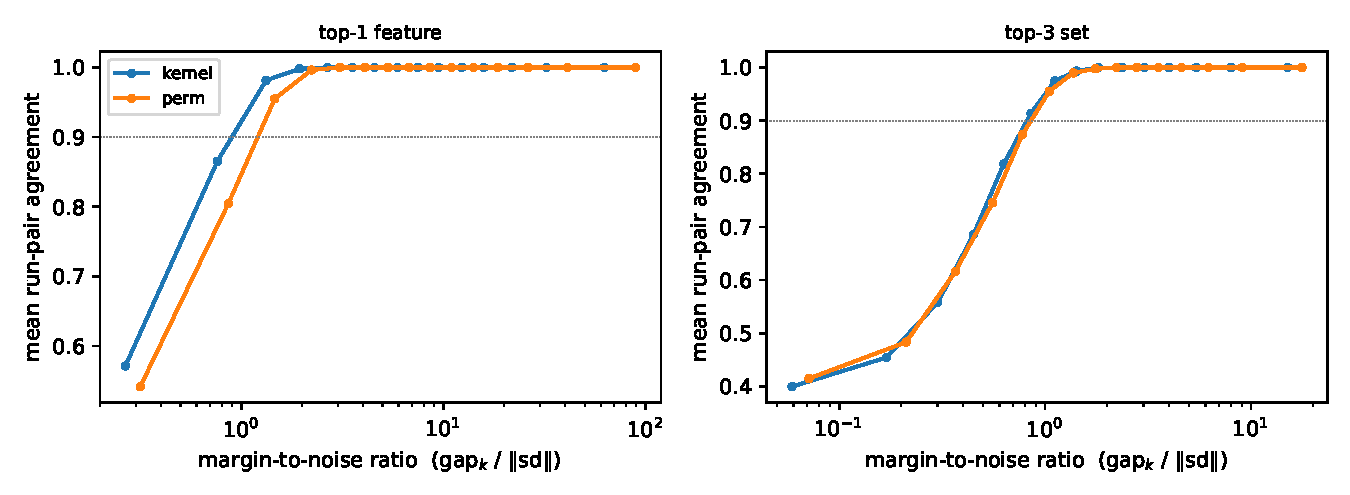
\includegraphics[width=\columnwidth]{fig_collapse.pdf}
\caption{Run-pair agreement vs.\ margin-to-noise ratio (binned quantiles of all non-exact configurations on the $d\le10$ datasets, budgets $m/d\ge4$). Agreement saturates near 1 once the ratio exceeds about 2 (top-1) or 1.5 (top-3), and the two estimators fall on essentially the same curve. The noise level is measured from the same runs, so this is a consistency check rather than a prediction.}\label{fig:collapse}
\end{figure}

\subsection{Compared with other sources of variation (C4)}
\Cref{fig:yard,tab:yard} compare, on the same instances, the top-3 Jaccard between two independent draws from each source (all other attributions exact; 3 datasets $\times$ 4 models; 100 instances, 30 for the background rows). Coalition-sampling noise at $16d$ (median Jaccard 0.94--0.95) is much smaller than model-retraining disagreement (0.68), than background resampling at $B{=}100$ (0.87) and than the value-function change for trees (0.75), and far above chance (0.45 for two different instances); paired by instance (Wilcoxon, Holm over 96 tests), sampling at $16d$ is more stable than retraining in 12/12 cells for both estimators and than $B{=}100$ background resampling in 8/12 (Kernel) and 6/12 (permutation) cells, and in no cell less stable. At $4d$ sampling noise (0.85--0.89) is still more stable than retraining in 8/12 (Kernel) and 12/12 (permutation) cells but comparable to background resampling at $B{=}100$ (more stable in 4/12 cells, less stable in 1/12). C4 is supported, with the qualification that background noise is comparable to sampling noise at small budgets. Fragility is partly an instance property: the per-instance top-3 Jaccard under Kernel and permutation at $4d$ is strongly rank-correlated (median Spearman 0.84, range 0.61--0.86 over 12 cells) but only weakly with that under retraining (median 0.24, range $-$0.03--0.71) or background draws (0.35, $-$0.06--0.78). Hence instances whose top-3 flips under sampling are not reliably the ones that flip under retraining: sampling noise is not a proxy for model-level ambiguity.

\begin{figure*}[t]
\centering
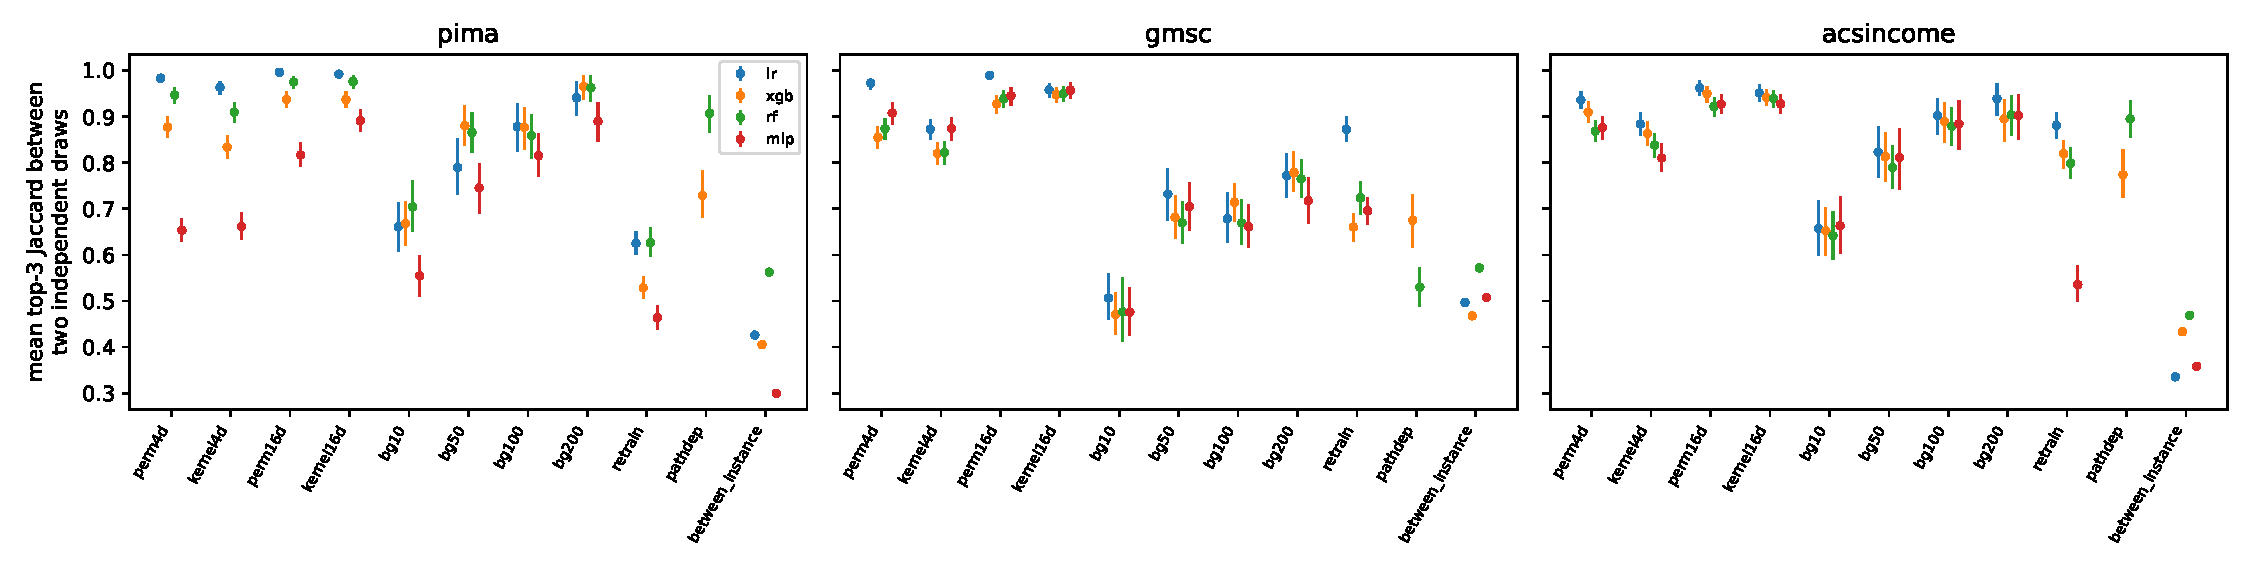
\includegraphics[width=\textwidth]{fig_yard.pdf}
\caption{Mean top-3 Jaccard (95\% bootstrap CI over instances) between two independent draws from each source of variability, by dataset and model. perm/kernel$k$d: coalition-sampling noise at $m=k\,d$ (fixed model and background); bg$B$: random backgrounds of size $B$ (exact attributions); retrain: bootstrap-retrained models; pathdep: path-dependent vs.\ interventional TreeSHAP (trees); between\_instance: two different instances (chance level).}\label{fig:yard}
\end{figure*}
\begin{table}[t]
\caption{Source comparison: median over cells (dataset$\times$model) of the cell-mean agreement, [min, max over cells].}\label{tab:yard}
\centering\scriptsize\setlength{\tabcolsep}{2.5pt}
\begin{tabular}{lcccc}
\toprule
Source of difference & cells & top-1 agree & top-3 Jaccard & rel.\ $\ell_2$\\
\midrule
Kernel sampling, $m=4d$ & 12 & 0.92 [0.72,0.97] & 0.85 [0.66,0.96] & 0.18\\
Permutation sampling, $m=4d$ & 12 & 0.93 [0.67,1.00] & 0.89 [0.65,0.98] & 0.11\\
Kernel sampling, $m=16d$ & 12 & 0.98 [0.93,1.00] & 0.95 [0.89,0.99] & 0.05\\
Permutation sampling, $m=16d$ & 12 & 0.97 [0.84,1.00] & 0.94 [0.82,1.00] & 0.06\\
Background resampling, $B=10$ & 12 & 0.63 [0.42,0.83] & 0.65 [0.47,0.70] & 0.51\\
Background resampling, $B=50$ & 12 & 0.86 [0.78,0.94] & 0.79 [0.67,0.88] & 0.24\\
Background resampling, $B=100$ & 12 & 0.88 [0.84,0.97] & 0.87 [0.66,0.90] & 0.20\\
Background resampling, $B=200$ & 12 & 0.95 [0.85,0.99] & 0.90 [0.72,0.97] & 0.12\\
Model retraining (bootstrap) & 12 & 0.74 [0.46,0.94] & 0.68 [0.46,0.88] & 0.44\\
Path-dep.\ vs.\ interventional TreeSHAP & 6 & 0.85 [0.71,0.93] & 0.75 [0.53,0.91] & 0.30\\
Two different instances (chance level) & 12 & 0.35 [0.17,0.59] & 0.45 [0.30,0.57] & 1.35\\
\bottomrule
\end{tabular}

\end{table}

\subsection{What a practitioner can do (C5)}\label{sec:cert}
\begin{table}[t]
\caption{Single-run certificate ($z\ge1.96$) from permutation runs, mean over four datasets, runs $\times$ instances $\times$ models pooled. acc.: fraction of runs whose top-1 (top-3 set) equals the exact (German: high-budget) reference; coverage: fraction certified; brackets: minimum over datasets.}\label{tab:cert}
\centering\scriptsize\setlength{\tabcolsep}{2.5pt}
\begin{tabular}{r|ccc|ccc}
\toprule
& \multicolumn{3}{c|}{top-1 feature} & \multicolumn{3}{c}{top-3 set}\\
$m/d$ & acc.\ (all) & coverage & acc.\ (cert.) & acc.\ (all) & coverage & acc.\ (cert.)\\
\midrule
4 & 0.93 & 0.78 & 0.98 [0.97] & 0.81 & 0.58 & 0.93 [0.90]\\
8 & 0.95 & 0.80 & 0.99 [0.99] & 0.86 & 0.58 & 0.98 [0.98]\\
16 & 0.96 & 0.85 & 1.00 [1.00] & 0.90 & 0.65 & 0.99 [0.99]\\
32 & 0.98 & 0.88 & 1.00 [1.00] & 0.93 & 0.72 & 1.00 [1.00]\\
\bottomrule
\end{tabular}

\end{table}
\Cref{tab:cert}: certified top-1 claims are right for 0.977 (at $m=4d$) to 0.999 ($32d$) of runs with 78--88\% coverage, against 0.93--0.98 unconditional; certified top-3 sets are right for 0.93--0.997 with 58--72\% coverage, against 0.81--0.93. The certificate thus identifies which single runs to trust without a second run, at the price of abstaining on 12--42\% of runs. Its minimum over datasets is 0.90 (top-3) and 0.97 (top-1) at $m=4d$. The reference for German is itself estimated, so accuracies there are slightly pessimistic. Splitting a budget (\cref{tab:split}): for permutation sampling, averaging 2 or 4 runs of budget $m/k$ gives the same error and top-3 accuracy as a single run of budget $m$ (error ratio 1.00--1.03), so repeat runs, hence an agreement check or a variance estimate, are free; for Kernel SHAP it is not (ratio 1.18--1.63, top-3 accuracy lower by 0.01--0.04), as the single larger run enumerates more of the strata. C5 holds in this setting.
\begin{table}[t]
\caption{Averaging $k$ runs of budget $m/k$ vs.\ one run of budget $m$ (pooled over cells where defined): median over cells of the per-cell median ratio of relative errors to the reference; mean top-3 accuracy.}\label{tab:split}
\centering\scriptsize\setlength{\tabcolsep}{3pt}
\begin{tabular}{llr|cc}
\toprule
Estimator & split & $m/d$ (each) & err.\ ratio (avg./single) & top-3 acc.\ avg./single\\
\midrule
Perm. & 2$\times$ & 4 & 1.00 & 0.86 / 0.86\\
Perm. & 2$\times$ & 8 & 1.00 & 0.90 / 0.90\\
Perm. & 2$\times$ & 16 & 1.01 & 0.93 / 0.93\\
Perm. & 4$\times$ & 4 & 1.00 & 0.90 / 0.90\\
Perm. & 4$\times$ & 8 & 1.03 & 0.93 / 0.93\\
Perm. & 4$\times$ & 16 & 1.03 & 0.96 / 0.96\\
Kernel & 2$\times$ & 4 & 1.38 & 0.82 / 0.87\\
Kernel & 2$\times$ & 8 & 1.19 & 0.90 / 0.92\\
Kernel & 2$\times$ & 16 & 1.18 & 0.94 / 0.95\\
Kernel & 4$\times$ & 4 & 1.63 & 0.88 / 0.92\\
Kernel & 4$\times$ & 8 & 1.40 & 0.93 / 0.95\\
Kernel & 4$\times$ & 16 & 1.58 & 0.96 / 0.98\\
\bottomrule
\end{tabular}

\end{table}

\section{Discussion and Limitations}\label{sec:limits}
\textbf{Verdict.} ``Is one run enough?'' depends on the question. (i) \emph{Which feature mattered most?} Usually yes at $\gtrsim16d$ (86--92\% of instances pass, pooled), when the background is fixed. (ii) \emph{Which three features?} Often no: even at $32d$--$64d$, 7--25\% of instances fail the 0.9 criterion for the top-3 set (pooled), concentrated in small-margin instances. (iii) Under the common practice of resampling the background, no, for either use. A deployer who must report a ranked list should fix and report the background, enumerate when $2^d\cdot B$ model calls are affordable, otherwise use permutation sampling at $\ge16d$, split the budget in two for a free agreement check, and abstain from top-$k$ claims when $z<1.96$.

\textbf{Limitations.} (1) \emph{Scope}: four datasets with $d\le20$ and four model classes (not FT-Transformer/ResNet \citep{gorishniy2021} or larger $d$); one ACS state; 100 (50) instances; one trained model for the main experiment (retraining enters only as a yardstick). (2) \emph{Value function}: marginal/interventional expectations with $B{=}100$ random background rows (a fixed $B$ in the main experiment; $B$ varies only in the yardstick experiment) and probability-scale outputs; conditional-expectation SHAP and other scales were not studied beyond a log-odds sensitivity check, where RF log-odds is affected by clipping. (3) \emph{Reference}: for $d{=}20$ the reference is an estimate, so accuracy-to-reference there is approximate and run--run metrics are the cleaner evidence. (4) \emph{Implementation}: the main experiment uses our re-implementation of the estimators (validated against shap at $m\ge4d$ on Pima only); shap's default $\ell_1$ feature selection for large $d$ is not reproduced; production configurations (other seeds/libraries, antithetic variants, Leverage SHAP) may differ. (5) \emph{Criterion}: the 0.9 pass threshold is a convention (ordering is robust in \cref{app:thr}); top-3 membership is a hard criterion that penalises benign near-tie swaps; we report RBO and $\tau$ for completeness. (6) The margin-to-noise AUC is not an independent predictor; the certificate is, but it was evaluated on the same instances as the rest (thresholds fixed in advance, no tuning). (7) Negative/inconclusive: no consistent boundary-proximity effect; no evidence on dependence on $d$ beyond German vs.\ the rest; Kernel vs.\ permutation shows no uniform winner. (8) Pooled CIs treat the 16 cells as exchangeable draws, which they are not; per-cell intervals are in the released tables.

\textbf{Conclusion.} A single SHAP run is a reliable basis for a coarse claim (the dominant feature, the overall ranking) when the background is fixed and the budget is $\gtrsim16d$ (or enumeration is affordable); it is not a reliable basis for the exact membership of a top-$k$ set, nor for any claim when the background is resampled between runs. Reliability is a property of the instance's margin relative to estimator noise, can be assessed from a single permutation run, and should be reported alongside the attribution.

\section*{Impact Statement}
This paper presents work whose goal is to advance the field of Machine Learning, specifically the reliability of feature-attribution explanations. Better calibrated use of SHAP in credit or medical contexts could reduce unjustified confidence in explanations; conversely the guidance here is limited to the tested settings and should not be read as certifying explanations as faithful or causal.

\bibliography{refs}
\bibliographystyle{icml2026}

\newpage
\appendix
\onecolumn
\section{Additional results and reproducibility}
\subsection{Models and data}\label{app:models}
Test AUC / accuracy of the models explained in the main experiment (70/30 stratified split, seed 0; training sets capped at 30k rows):

\begin{center}\small\begin{tabular}{lcccc}
\toprule
Dataset ($d$) & LR & XGB & RF & MLP\\
\midrule
Pima (8) & 0.872 / 0.771 & 0.825 / 0.771 & 0.851 / 0.784 & 0.800 / 0.740\\
GMSC (10) & 0.851 / 0.938 & 0.859 / 0.937 & 0.855 / 0.937 & 0.858 / 0.936\\
ACSIncome (10) & 0.855 / 0.775 & 0.872 / 0.788 & 0.858 / 0.776 & 0.864 / 0.781\\
German (20) & 0.806 / 0.760 & 0.808 / 0.763 & 0.818 / 0.760 & 0.734 / 0.707\\
\bottomrule
\end{tabular}
\end{center}
Pima: OpenML id 37; GMSC: OpenML id 46929 (150k rows, median imputation); ACSIncome: folktables 2018 1-year person file, Colorado (31,306 rows after the standard filter); German: UCI Statlog (1,000 rows; ``bad credit'' is the adverse class). Trees use integer-coded categories (code = training-frequency rank, rare levels merged); LR/MLP use one-hot features and winsorised standardised numerics. Attribution players are the original attributes.

\subsection{Validation against shap and Kernel conditioning}\label{app:valid}
\begin{center}\small\begin{tabular}{r|cc|cc}
\toprule
& \multicolumn{2}{c|}{Kernel RMSE} & \multicolumn{2}{c}{Permutation RMSE}\\
$m$ & ours & \texttt{shap} & ours & \texttt{shap}\\
\midrule
32 & 0.0130 & 0.0132 & 0.0079 & 0.0076\\
64 & 0.0062 & 0.0061 & 0.0055 & 0.0054\\
128 & 0.0034 & 0.0036 & 0.0039 & 0.0039\\
\bottomrule
\end{tabular}
\hspace{2em}\begin{tabular}{rrrr}
\toprule
$d$ & $m/d$ & $m$ & frac.\ ill-conditioned\\
\midrule
8 & 2 & 16 & 0.137\\
8 & 3 & 24 & 0.007\\
8 & 4 & 32 & 0.000\\
8 & 8 & 64 & 0.000\\
10 & 2 & 20 & 0.227\\
10 & 3 & 30 & 0.003\\
10 & 4 & 40 & 0.000\\
10 & 8 & 80 & 0.000\\
20 & 2 & 40 & 0.163\\
20 & 3 & 60 & 0.003\\
20 & 4 & 80 & 0.003\\
20 & 8 & 160 & 0.000\\
\bottomrule
\end{tabular}
\end{center}
Left: median over models/instances of RMSE to exact Shapley values (Pima, 100 runs), ours vs.\ the shap package at equal evaluation budget (for the permutation explainer, \texttt{max\_evals}$=m+2d$). Right: fraction of 300 random Kernel designs whose normal matrix has condition number $>10^8$ (\texttt{code/check\_singular.py}).

\subsection{Pass-criterion threshold}\label{app:thr}
\begin{center}\small\begin{tabular}{lr|cccc|cccc}
\toprule
& & \multicolumn{4}{c|}{top-1 pass rate at threshold} & \multicolumn{4}{c}{top-3 set pass rate at threshold}\\
est. & $m/d$ & 0.80 & 0.90 & 0.95 & 0.99 & 0.80 & 0.90 & 0.95 & 0.99\\
\midrule
kernel & 4 & 0.79 & 0.74 & 0.69 & 0.64 & 0.44 & 0.35 & 0.29 & 0.24\\
kernel & 8 & 0.89 & 0.86 & 0.83 & 0.81 & 0.64 & 0.57 & 0.53 & 0.49\\
kernel & 16 & 0.94 & 0.92 & 0.90 & 0.89 & 0.76 & 0.71 & 0.67 & 0.64\\
kernel & 32 & 0.98 & 0.97 & 0.96 & 0.95 & 0.89 & 0.85 & 0.82 & 0.81\\
\midrule
perm & 4 & 0.79 & 0.75 & 0.71 & 0.69 & 0.54 & 0.48 & 0.44 & 0.41\\
perm & 8 & 0.84 & 0.81 & 0.78 & 0.76 & 0.65 & 0.59 & 0.54 & 0.51\\
perm & 16 & 0.89 & 0.86 & 0.84 & 0.82 & 0.73 & 0.68 & 0.63 & 0.60\\
perm & 32 & 0.93 & 0.90 & 0.88 & 0.87 & 0.79 & 0.75 & 0.73 & 0.70\\
\bottomrule
\end{tabular}
\end{center}

\subsection{Additional main-experiment results}\label{app:more}
\textbf{Frontier} (smallest $m/d$ from which the pass rate stays $\ge0.9$ in the grid; $>$ means not reached):
\begin{center}\small\begin{tabular}{llcccc}
\toprule
& & \multicolumn{2}{c}{top-1: min.\ $m/d$} & \multicolumn{2}{c}{top-3 set: min.\ $m/d$}\\
Dataset & model & Kernel & Perm. & Kernel & Perm.\\
\midrule
Pima & lr & 4 & 4 & 8 & 4\\
 & xgb & 16 & 64 & 32 & $>$64\\
 & rf & 8 & 4 & 32 & 32\\
 & mlp & 32 & $>$64 & 32 & $>$64\\
\midrule
GMSC & lr & 4 & 2 & 64 & 8\\
 & xgb & 8 & 16 & 64 & $>$64\\
 & rf & 16 & 16 & 64 & $>$64\\
 & mlp & 8 & 8 & 64 & $>$64\\
\midrule
ACSIncome & lr & 16 & 8 & 64 & $>$64\\
 & xgb & 16 & 32 & $>$64 & $>$64\\
 & rf & 32 & 64 & $>$64 & $>$64\\
 & mlp & 16 & 32 & $>$64 & $>$64\\
\midrule
German & lr & 16 & 8 & 16 & $>$32\\
 & xgb & 16 & 32 & $>$32 & $>$32\\
 & rf & 8 & 8 & $>$32 & $>$32\\
 & mlp & $>$32 & $>$32 & $>$32 & $>$32\\
\bottomrule
\end{tabular}
\end{center}
\textbf{AUCs} for predicting pass at $m/d\ge4$, non-exact:
\begin{center}\small\begin{tabular}{llccccc}
\toprule
Est. & target & margin/noise & gap only & $-$non-add. & budget only & base rate\\
\midrule
kernel & pass1 & 1.00 & 0.92 & 0.67 & 0.74 & 0.90\\
kernel & pass3 & 0.99 & 0.85 & 0.65 & 0.72 & 0.65\\
perm & pass1 & 1.00 & 0.92 & 0.66 & 0.65 & 0.87\\
perm & pass3 & 0.99 & 0.86 & 0.66 & 0.65 & 0.70\\
\bottomrule
\end{tabular}
\end{center}
\textbf{Probability vs.\ log-odds value function} (pass rates, $d\le10$ datasets):
\begin{center}\small\begin{tabular}{llr|cc|cc}
\toprule
& & & \multicolumn{2}{c|}{top-1 pass} & \multicolumn{2}{c}{top-3 pass}\\
model & est. & $m/d$ & prob. & log-odds & prob. & log-odds\\
\midrule
lr & kernel & 4 & 0.90 & 1.00 & 0.56 & 1.00\\
 & kernel & 16 & 0.95 & 1.00 & 0.83 & 1.00\\
 & perm & 4 & 0.92 & 1.00 & 0.81 & 1.00\\
 & perm & 16 & 0.96 & 1.00 & 0.91 & 1.00\\
\midrule
xgb & kernel & 4 & 0.74 & 0.88 & 0.31 & 0.54\\
 & kernel & 16 & 0.95 & 0.97 & 0.68 & 0.84\\
 & perm & 4 & 0.76 & 0.94 & 0.43 & 0.76\\
 & perm & 16 & 0.87 & 0.96 & 0.68 & 0.89\\
\midrule
rf & kernel & 4 & 0.76 & 0.61 & 0.39 & 0.22\\
 & kernel & 16 & 0.92 & 0.82 & 0.74 & 0.58\\
 & perm & 4 & 0.77 & 0.62 & 0.50 & 0.26\\
 & perm & 16 & 0.88 & 0.76 & 0.72 & 0.49\\
\midrule
mlp & kernel & 4 & 0.67 & 0.73 & 0.25 & 0.43\\
 & kernel & 16 & 0.91 & 0.91 & 0.65 & 0.73\\
 & perm & 4 & 0.67 & 0.74 & 0.35 & 0.54\\
 & perm & 16 & 0.82 & 0.84 & 0.55 & 0.72\\
\bottomrule
\end{tabular}
\end{center}
\textbf{Rank metrics} (RBO, Kendall $\tau$, Jaccard$@5$, relative $\ell_2$), per-cell tables, boundary-proximity tests and Kernel-vs-permutation tests are in \texttt{results/tables/} (\texttt{tabA}--\texttt{tabM}).

\subsection{Reproducibility and checklist}\label{app:repro}
Code, commands, library versions, seeds and estimated runtimes are in the supplementary \texttt{README.md}; every table and figure is produced by the script listed there. Measured CPU time: main experiment 1.9 h, yardsticks 1.4 h, default-shap experiment 1.1 h; validation and analysis scripts were not separately logged (estimated $<0.6$ h), i.e.\ $\approx$ 5 CPU-hours in total on a shared host (no GPU). The ICML 2026 template has no mandatory checklist; we nevertheless state: claims match the evidence reported (see Limitations); all code and results are released; no human subjects; datasets are public (German: CC BY 4.0; ACS PUMS: US Census public data; OpenML sets: licence ``Public''); no new data collected.

\end{document}
